\chapter{Introduzione}

Un Lexer $\lambda $ \'e un DFA, ogni stato finale $\phi _i$ \'e associato ad una regular expression $\alpha _i$.
Una stringa $s \in L(\lambda )$, il pattern matching termina in uno stato finale $\phi _j$ ed s \'e associata ad una regular expression 
$\alpha _j$; token: ($s, \alpha _j$).

\begin{center}
	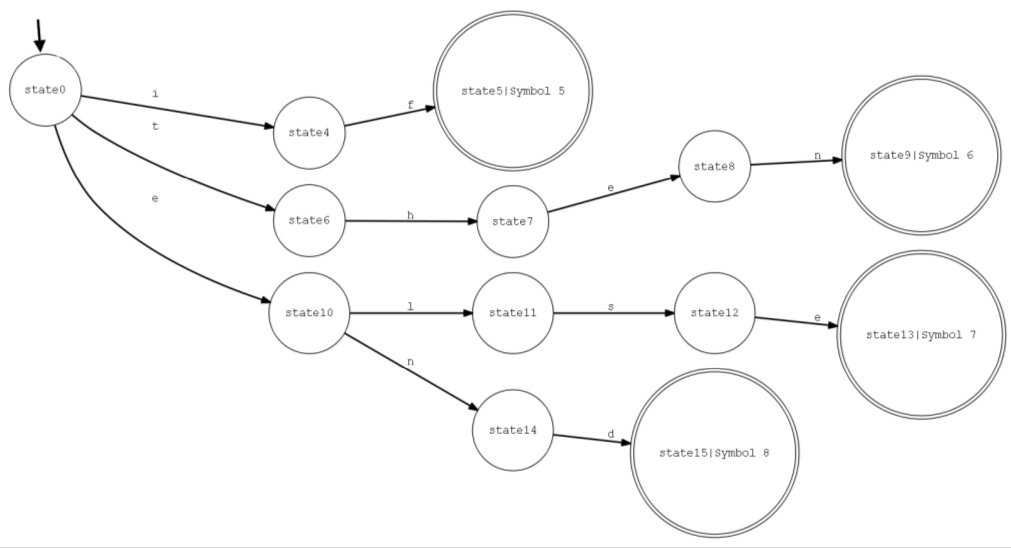
\includegraphics[scale=0.35]{Chapters/Img/c01_01.png}\\
\end{center}
	

\begin{itemize}
	\item (if, 5) \\
	\item (then, 6)\\
	\item (else, 7)\\
	\item (end, 8)\\
\end{itemize}

Data la descrizione del linguaggio che vuoi matchare lui ti genera il codice C per farlo. 

\section{Get started}
\begin{tabular}{ll}
	Windows & https://sourceforge.net/projects/winflexbison/ \\
	Linux & sudo apt-get install bison flex gcc\\
	Mac & XCode
\end{tabular}

\chapter{FLEX (Fast Lex)}

Posso annotare una regular expression con istruzioni C.

\section{Lex matching character}

\subsection{Operatori}
\begin{tabular}{ll}
	$\alpha \cdot \beta$ 			& 	concatenazione\\
	$\alpha | \beta$ 				& 	alternazione\\
	$\alpha +$ 						& 	1+ ripetizioni\\
	$\alpha *$ 						& 	0+ ripetizioni\\
	$\alpha ?$ 						&	0 o 1 ripetizione\\
	.       						&	un carattere qualsiasi (tranne $\backslash$n) \\
	$\alpha \{n,m\}$ 				& 	$(n \leq m)$ matches $\alpha$ from n to m times\\
	$[a-z]$   						&	intervallo di caratteri da \lq a \rq\ a \lq z \rq \\
	$[0-9a-z\_]*$  					&	(intervalli multipli) considerati 0+ volte [tutti gli id] \\
	\hline
	$a\$ $ 							& 	\lq a\rq\ a fine di una linea \\
	$\text{\textasciicircum}a$  							& 	\lq a\rq\ all'inizio di una linea \\
	$<<EOF>>$ 						&	\\
	\hline
	$a/b$ 							& 	\lq a\rq\ iif \lq b\rq\ segue \\ 
	$[\text{\textasciicircum}C]$ 	&	complementare \\
	$[\text{\textasciicircum}CB]$	&	$= [\text{\textasciicircum}C\text{\textasciicircum}B]$ matcha bat ma non Bat o Cat \\
	\hline
	$"stringa"$						& 	\\
	$."at"$							&	matches words: \lq\lq cat\rq\rq , \lq\lq rat\rq\rq , etc.\\
\end{tabular}

\section{Template Lex}
\begin{lstlisting}
	%{ 
		/* Dichiarazioni iniziali in codice C (librerie e variabili globali) */	
	%}

	/* " Named " regular expressions here . */

	%%
	/* " Anonymous " Regular expressions here . */
	%%
	
	/* This section is copied verbatim into the lexer 's source . */
\end{lstlisting}

Nel primo blocco posso ficcare istruzioni C che verranno copiate verbatim (pari pari) nel sorgente C; ad esempio posso dichiarare 
variabili che poi uso nelle \textbf{semantic actions} delle regex.

Nel secondo blocco posso dare un nome ad una regex (al uso nella sezione 
dopo con l'operatore $\{ \}$):

\begin{lstlisting}
	%{ /* Copied verbatim in lexer 's source . */ %}

	Type ( " int " | " float " )
	%%
	{ Type } 	{ /* A Semantic action . */ }
	[a - z ]+ 	{ /* Another one . */ }
	%%

	int yywrap () { 
		return 1;	//if I find eof should stop lexing?
	}

	int main ( int iArgC , char ** lpszArgV ) {
		yylex (); 	// Starts lexing .
	}
\end{lstlisting}

\section{Compilare}

\begin{lstlisting}
	> flex Input.l
	> gcc lex.yy.c -o Lexer.out -std=c99
	> Lexer.out < In.txt
\end{lstlisting}

\section{Variabili generate da Lex}
\begin{lstlisting}
	FILE * yyin ;		/* Default value is stdin . */
	FILE * yyout ;		/* Default value is stdout . */
	int yyleng ;		/* Number of characters read . */
	char * yytext ;		/* The buffer on which characters are copied during pattern matching*/
\end{lstlisting}

\subsection{Esempi Regex}

\begin{lstlisting}
	%{
		#include <stdlib.h>
		int iWords = 0;
	%}

	word	[^ \t\r\n]
	Declaration				"public"[ \t]+("static"[ \t]+)?"void"[ \t]+"main"

	%%

	{word}			{iWords+=1;}
	{Declaration} 	{printf("siamo nel main feghio")}
	.|\n			{printf(" %d ", n++); /*mi stampa il numero di caratteri*/} 
	.|\n			{ECHO; /* mi stampa l'ultima parola per intero */} 

	"if"		|
	"else"		|
	"for"			{fprintf(stdout, "This is a keyword: %s\n", yytext);}

	[\t \n\r]+		{/*Do nothing.*/;}
	.|\n			{ECHO; fprintf(stdout, " is not a keyword.\n");}

	<<EOF>>			{printf("words: %d \n", iWords); return yytext[10];}

	%%

	int yywrap() { 
		return 1; //true per input multipli 
	}

	int main() {
		printf("%d", yylex()); //10
	}

\end{lstlisting}

\subsection{Yywrap Function}

When the scanner receives an end-of-file indication from YY$\_$INPUT, it then checks the yywrap() function. 
If yywrap() returns false (zero), then it is assumed that the function has gone ahead and set up yyin to point to another input file, 
and scanning continues. If it returns true (non-zero), then the scanner terminates, returning 0 to its caller. 
Note that in either case, the start condition remains unchanged; it does not revert to INITIAL. 

\subsection{Input Multipli}
\begin{lstlisting}
	%{
		#include <stdlib.h>
		int iCurrentFile = 0;
		int iFiles = 0;
		char**lpszFileName = NULL;
	%}
	%%
	.|\n 	{printf("ciao"):}
	%%
	int yywrap() {
		FILE*fInput = NULL;
		if (iCurrentFile<iFiles) {
			printf("Frase finale");
			//reset variables

			fclose(yyin);

			iCurrentFile+=1;

			fInput = fopen(lpszFileName[iCurrentFile], "r");
			if (fInput!=NULL) {
				yyin = fInput; //yyin il file da parsare
			}		
		}
		return fInput!=NULL ? 0 : 1;
	}

	int main(int iArgC, char**lpszArgV) {
		if (iArgC>1){
			iFiles=iArgC;
			lpszFileName = &lpszArgV[1];

			FILE*fInput = fopen(lpszFileName[iCurrentFile], "r");
			if (fInput!=NULL) {
				yyin = fInput; 
				yylex(); //start parsing yyin
			}
		}
	}
\end{lstlisting}

\section{Context Sensitivity (CS)}
In base al token letto devo comportarmi in modo diverso.
Ho delle \textbf{start conditions} (o start state), solo una \'e attiva. Il primo start state \'e l'\textbf{initial}.
Uno start state pu\'o essere \textbf{inclusivo} o \textbf{esclusivo}.

Da uno start state esclusivo solo regex correlate ad esso sono raggiungibili.

Da uno start state inclusivo tutte le regex correlate ad esso ed anche quelle non correlate agli altri start state sono raggiungibili.

\begin{lstlisting}
	%{ /* */ %}

	% x String 	// Exclusive start states
	% s Cond 	// Inclusive start states

	%%
	...
	%%
\end{lstlisting}

\section{Associare regole a stati}
Per assegnare uno start state ad una re uso \textbf{$<$NOME SS$>$}.
Per entrare in uno stato uso il comando \textbf{BEGIN}.
All inizio il lexer \'e nello stato \textbf{INITIAL}.
\begin{lstlisting}
	%{ /* */ %}

	% x Cond
	
	%%
	" \" "				{ /* Read " char . */ BEGIN Cond ;}
	< Cond >(^[ " ])+	{ /* Consume string content . */ }
	< Cond > " \" "		{ /* Read " char . */ BEGIN INITIAL ;}
	%%
\end{lstlisting}

\subsection{Stati inclusivi ed esclusivi}
\begin{lstlisting}
	%{ /* EXCLUSIVE START STATE*/ %}

	%x String Unreacheable

	%%
	" \" "					{ /* Read " char . */ BEGIN String ;}
	< String > (^[ " ])+	{ /* Consume string content . */ }
	< String > " \" "		{ /*Read " char . */ BEGIN INITIAL ;}
	< Unreacheable > "end"	{ /* Will never be matched . */ }
	%%

	%{ /* INCLUSIVE START STATE */ %}
	
	%s String
	
	%%
	" \" " 				{ /* Read " char . */ BEGIN String ;}
	< String >(^[ " ])+	{ /* Consume string content . */ }
	< String > " \" " 	{ /* Read " char . */ BEGIN INITIAL ;}
	" end "				{ /* Will be matched . */ }
	%%
\end{lstlisting}
Gli start state sono realizzati tramite uno stack, ho tre funzioni per manipolarli:
\begin{itemize}
	\item void yy push state(int NewState) //pusho in cima allo stack, equivalente a BEGIN NewState;\\
	\item void yy pop state() //fa una pop, equivalente a BEGIN;\\
	\item int yy top state() //fa la top, non esistono metacomandi per farla;\\
\end{itemize}

\subsection{Esempio}

\begin{lstlisting}
%{
    #include <stdlib.h>

    int iLine = 0;
    int iColumn = 0;
%}

%s FirstDate 
%x SecondDate Motivation Amount Info

%%

"#".+		{iColumn+=yyleng;}

"$"		{iColumn+=1; 
			fprintf(yyout, "INSERT INTO Movement(SDate, EDate, Desc, Amount, Info) VALUES (");
			BEGIN FirstDate;}

([0-9]{2}"/"?){3}					{iColumn+=yyleng; 
										fprintf(yyout, "to_date('%s', 'DD/MM/YY'), ", yytext); 
										BEGIN SecondDate;}

<SecondDate>([0-9]{2}"/"?){3}	{iColumn+=yyleng;
										fprintf(yyout, "to_date('%s', 'DD/MM/YY'), ", yytext); 
										BEGIN Motivation;}

<Motivation>[^-0-9]+                {iColumn+=yyleng;
                                    fprintf(yyout, "'%s', ", yytext); BEGIN Amount;}

<Amount>"-"?[0-9\.]+","[0-9]{2}[ \t]+"EUR"        {int i=0, j=0;
                                                    for (;i<yyleng; i+=1, j+=1) {
                                                        if (yytext[i]=='.') {
                                                            i+=1;
                                                        }
                                                        if (i!=j) {
                                                            yytext[j]=yytext[i];
                                                        }
                                                    }
                                                    yytext[j]='\0';
                                                    for (int i=0; i<yyleng; i+=1) {
                                                        if (yytext[i]==','){yytext[i]='.';}
                                                        if (yytext[i]==' '){
                                                            yytext[i]='\0'; break;
                                                        }
                                                    }
                                                    fprintf(yyout, "%s, ", yytext);
                                                    BEGIN Info;}

<Info>[^$]*                         {for (int i=0; i<yyleng; i+=1) {
                                            if (yytext[i]=='\n'||yytext[i]=='\r') {
                                                yytext[i]=' ';
                                            }
                                        }
                                        fprintf(yyout, "'%s');\n", yytext);
                                        BEGIN INITIAL;}

[ \t]+                              {iColumn+=yyleng;}
[\r\n|\r|\n]                        {iColumn=0; iLine+=1;}
.                                   {printf("ERROR in line: %d, column: %d.", iLine, iColumn); 
										yyterminate();}
%%

int yywrap(){return 1;}

int main(int iArgC, char**lpszArgV) {
    FILE*fInput = fopen(lpszArgV[1], "r");
    FILE*fOutput = fopen(lpszArgV[2], "w");
    if (fInput!=NULL && fOutput!=NULL) {
        yyin = fInput;
        yyout = fOutput;

        fprintf(yyout, "DROP TABLE IF EXISTS Movement;");
		fprintf(yyout, "CREATE TABLE Movement(\n\tStartDate DATE,\n\tEndingDate DATE, ...;\n");
        yylex();
    }
}
\end{lstlisting}

\section{Ambiguous Specifications}
Dati $\alpha$ e $\beta$ regular expressions talich\'e $L(\alpha ) \subset L(\beta )$, devo stare attento all'ordine in cui le scrivo, quelle pi\'u in alto hanno precedenza su quelle pi\'u in basso. 

\begin{tcolorbox}\begin{center}
	Se con molte regular expression posso arrivare in un nodo, vince quella a priorit\'a maggiore.
	Regular expressions generating constant finite languages must be placed first, or they will be obscured.
\end{center}\end{tcolorbox}

Una volta che una stringa \'e matchata viene \textbf{consumata}, le altre re non la potranno pi\'u matchare. 
Posso anche usare \textbf{REJECT} per darla in pasto alla seconda re in ordine di priorit\'a.

\begin{lstlisting}

	%{ int iCounter = 0; %}

	%%
	" abcde "	{ iCounter +=1; REJECT ;}
	" abcd "	{ iCounter +=1; REJECT ;}
	" abc "		{ iCounter +=1; REJECT ;}
	" ab "		{ iCounter +=1; REJECT ;}
	"a"			{ iCounter +=1; }
	.			{ /* Consumes the rest . */ }
	%%

	int main (){
		yylex ();
		/* iCounter = 5 when input is " abcde ". */
	}
\end{lstlisting}

\chapter{Exercises}
\section{Lex}

Devise a lexer accepting a Windows file path.\\
Devise a lexer accepting a Linux file path.\\
Devise a lexer accepting a non regular language.\\

\section{Yacc}

Design an unambiguous grammar for arithmetic expressions whose
operations are: difference, sum, product, division, exponentiation.\\
Remember to encode precedence and associativity:
Difference and sum are left associative.\\
Product, division and exponentiation are right associative.\\
